\chapter{Concluzii}


\indent\indent Verificarea programului \texttt{Monocypher} folosind \texttt{Eva} în \texttt{FramaC}
a evidențiat puterea pe care o are interpretarea abstractă în ce privește analiza
statică a valorilor variabilelor dintr-un program complex.

Pentru versiunea concretă a programului studiat, următoarele mențiuni sînt esențiale:
\begin{itemize}
\item În versiunile dinaintea \texttt{0.3}, programul conținea atît scurgeri de
  memorie, cît și neterminare. Cazul a fost analizat chiar de echipa \texttt{FramaC} și
  expus la \cite{framatut}, dar și de autor, pe pagina personală \cite{loupcrypto}.
  Eroarea este raportată printre mesaje ca în figura \ref{fig:nonterm0}, iar detaliile
  se pot accesa prin concentrarea pe această eroare (click dreapta, \texttt{Focus on this callstack}),
  ca în imaginea din figura \ref{fig:nonterm} (ambele imagini preluate din
  \cite{framatut}). Tot la \cite{framatut}
  sînt sugerate și idei de analiză a codului care să rezolve această problemă sau
  măcar să afle cît mai precis cauza.
\item În versiunea actuală (\cite{gh1}), programul nu mai conține bug-uri detectabile
  de \texttt{Eva}. De fapt, chiar autorul a inclus o serie de testuri și un script
  care rulează \texttt{frama-c} pe toate sursele C ale programului, rezultatul
  final fiind perfect, fără niciun mesaj de eroare, alarmă sau atenționare.
\end{itemize}


\begin{figure}[!htbp]
  \centering
  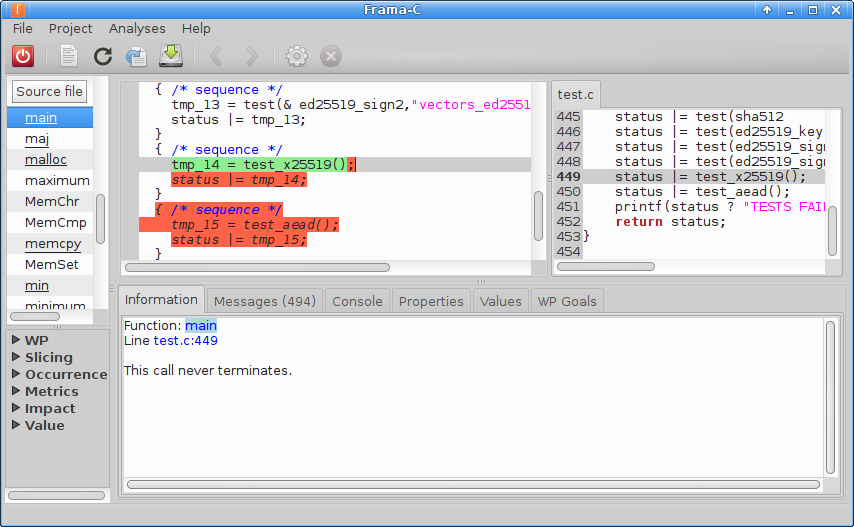
\includegraphics[width=0.7\textwidth]{img/nonterm0}
  \caption{Neterminarea din \texttt{Monocypher<0.3}}
  \label{fig:nonterm0}
\end{figure}


\begin{figure}[!htbp]
  \centering
  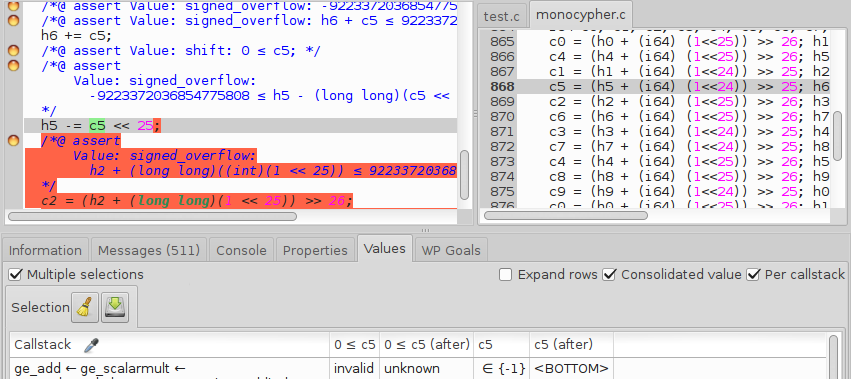
\includegraphics[width=0.8\textwidth]{img/nonterm}
  \caption{Detalii asupra neterminării din \ref{fig:nonterm0}}
  \label{fig:nonterm}
\end{figure}



%%% Local Variables:
%%% mode: latex
%%% TeX-master: "../mono-frama"
%%% End:
